\documentclass[oneside]{ausarbeitung}
\bibliography{latexlit}


% ----------------------------------------------------------------------

\begin{document}

%--- Language selection
% Allowed values:
%   \selectlanguage{english}
%   \selectlanguage{ngerman}
\selectlanguage{english}

%--- Type of paper
% Allowed values:
%   \Praxissemesterbericht
%   \Projektbericht
%   \Bachelorarbeit
%   \Seminararbeit
%   \Masterarbeit

\Bachelorarbeit

%--- Degree program:
% Allowed values:
%   \IN % Computer Science (Bachelor/Master)
%   \Elektronik
%   \AI % Artificial Intelligence and Data Science (Bachelor)
%   \MLD % Machine Learning and Data Analytics (Master)
\IN

\title{Title of the Paper}

\author{Jon Doe}
\matrikelnr{12345}

%--- Is the first supervisor (\examinerA) at the university a professor?
% Allowed values:
%   \examinerIsAProfessortrue   % Yes
%   \examinerIsAProfessorfalse  % No
\examinerIsAProfessortrue   % Yes

%--- Supervisors
\examinerA{Prof.~Dr.~Rainer~Werthebach}
%\examinerB{Prof.~Dr.~Ulrich~Klauck}

%--- Submission date
\date{20 June 2024}

%--- Company information
% Comment out if the paper was not written at an external company.
\companyname{Example Company}
\industrialsector{Example Industry}
\department{Example Department}
\companystreet{Example St. 1}
\companycity{12345 Sample City}

%--- Information about the supervisor at this company
\advisorname{Name of Supervisor}
\advisorphone{(01234) 567-890}
\advisoremail{name@company.xxx}

%--- Display title page
\maketitle
\cleardoublepage

%---
\pagenumbering{roman}
\setcounter{page}{1}

%--- Display company data
% Comment out if the paper was not written at an external company.
\makeworkplace
\cleardoublepage

%--- Display declaration of authorship
\makeaffirmation
\cleardoublepage

%--- Confidentiality clause (Only works for external bachelor's or master's theses.)
\makeconfidentialclause
\cleardoublepage

%---
\begin{abstract}
  The purpose of the abstract is to inform a reader (who may be in a hurry) so
  that they can decide whether the report is useful to them or not
  (in modern business terms: management summary). The abstract therefore provides
  a short presentation

  \begin{itemize}
    \item of the problem addressed in the paper
    \item of the method(s) used
    \item of the progress achieved in the paper.
  \end{itemize}

  It should not discuss the structure of the paper, i.e.
  Chapter~\ref{cha:grundlagen}, etc., because the abstract is intended to convey
  the most important aspects of the paper without requiring it to be read.
  A chapter-related presentation should appear in Chapter~%
  \ref{cha:einleitung} under approach.

  Length: Maximum 1 page.
\end{abstract}
%-----------------------------------------------------------------------
\cleardoublepage
\tableofcontents

%---
\listoffigures

%---
\listoftables

%---
\lstlistoflistings

%---
\listofabbreviations
\begin{acronym}[Ex.]  % Longest abbreviation in the following
                      % list to determine the width of the column for
                      % abbreviations.

%% Entry: \acro{reference name}[abbreviation]{full form}
%% In the text, the abbreviation is then used with \ac{reference name}.
\acro{rup}[RUP]{Rational Unified Process}
%\acro{bsp}[Ex.]{Example}
\end{acronym}
%---


\cleardoublepage
\pagenumbering{arabic}
\setcounter{page}{1}

% ----------------------------------------------------------------------
\chapter{Introduction}
\label{cha:einleitung}

The introduction serves to arouse the reader's interest in the contents
of the practical-semester report, to point out the problems dealt with,
and to describe the concepts developed to solve them.

\section{Motivation}
\label{sec:motivation}

The motivation explains the significance that the solutions to be developed
in the practical semester have for the supervising company.
For example, it shows which product they will become part of,
which process is to be improved, etc.

\section{Problem Statement and Delimitation}
\label{sec:problemstellung}

The problem statement serves to clearly define and delimit the problem to be solved.
The intern should have a clear understanding of the problem to be solved.
In particular, it should also prevent too many problems from being tackled at the same time.
A negative delimitation prevents expectations from being raised in the reader
that are later not fulfilled.

\section{Objective of the Paper}
\label{sec:ziel}

The objective of the paper defines the intended scope of the solution. It is based on this objective that it is decided whether the internship was successfully completed or not.

\section{Approach}
\label{sec:vorgehen}

After the problem statement and objective have, in a sense, described the starting point and endpoint
of the internship, the path taken to achieve the objective is presented here.
For this purpose, the following chapters and their contribution to achieving the objective of the paper
are typically described briefly. The following chapters represent one possible structure;
deviations may certainly be necessary. To present the approach, a graphical representation is useful,
showing the individual solution steps and their relationships.

%\begin{figure}[htbp]
%  \centering
%  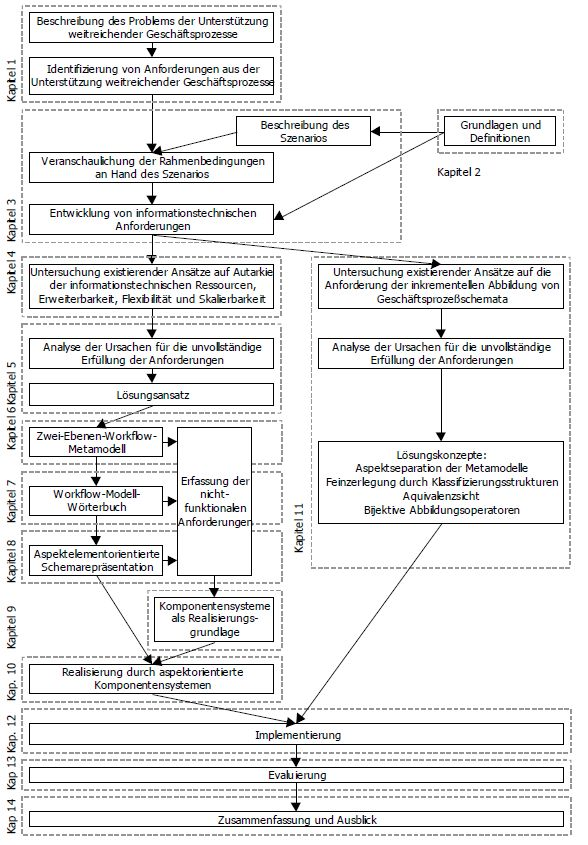
\includegraphics[height=0.9\textheight]{images/ausarbeitung.jpg}
%  \caption{approach according to \autocite{Schmidt:Geschaeftsprozesse}}
%  \label{fig:1}
%\end{figure}


% ---
\chapter{Fundamentals}
\label{cha:grundlagen}

This chapter presents the fundamental knowledge relevant to the internship.
The intern should present the theoretical knowledge known from lectures
or deepened through research that is necessary to solve the problems posed during the internship.

Care must be taken to include only content in the fundamentals chapter
that will also be used later (problem relevance).
Likewise, care must be taken to ensure that the fundamentals are presented
with sufficient depth and completeness.

The JabRef tool\autocite{JabRef:JabRef} is used to create the bibliography.

However, you can also use the Citavi tool\autocite{SAS:Citavi}
and export to \textsc{Bib}\TeX{} there.

\section{Fundamental Area A}
\label{sec:grundlagengebieta}

\blindtext

\subsection{Definition AA}
\label{sub:definitionaa}

\blindtext

\subsection{Definition AB}
\label{sub:definitionab}

\blindtext

\section{Fundamental Area B}
\label{sec:grundlagengebietb}

\blindtext

\subsection{Definition BA}
\label{sub:definitionBa}

\blindtext

\subsection{Definition BB}
\label{sub:definitionbb}

\blindtext

%---
\chapter{Problem Analysis}
\label{cha:problemanalyse}

The analysis of the problem to be solved is the foundation of every
engineering-based approach. Therefore, this chapter should analyze the
problem to be solved on the basis of the knowledge prepared in the fundamentals chapter.
For this purpose, it is particularly necessary to clarify how
the overall problem can be decomposed into subproblems and which
dependencies exist between them.

In software projects, this is typically where the
requirements analysis of the \ac{rup} is located.

%---
\chapter{Solution Concept}
\label{cha:loesungskonzept}

On the basis of the problem analysis prepared in the previous chapter
and the theoretical knowledge developed in the fundamentals chapter,
a solution concept is developed.

In software projects, this chapter typically corresponds to the
analysis and design phase of the \ac{rup}. Typical results of this phase are
class diagrams, etc.

%---
\chapter{Implementation}
\label{cha:implementierung}

This chapter describes the concrete implementation of the solution concept
developed in Chapter \ref{cha:loesungskonzept}.
Reference is made here to the specifically used development tools, etc.

In software projects, this chapter typically consists of the
implementation and test phases in the \ac{rup}.

For example, you can also include a small listing here (see \ref{lst:test}).

\begin{lstlisting}[language=c,%
                   caption={Heading of the Source Code},label=lst:test]
#include<stdio.h>

int main() {
    // Comment
    int answer = 20 << 1;
    answer += 2;
    printf("Halloechen Welt!\n");
    printf("The answer is: %d\n", answer);
    return 0;
}
\end{lstlisting}

Sometimes a small table also helps:

\begin{table}[htbp]
\centering
\begin{tabular}{|l|r|}
\hline
\textbf{Measured value a} & \textbf{Measured value b} \\ \hline
9 & 5 \\ \hline
1 & 4 \\ \hline
1 & 3 \\ \hline
\end{tabular}
\caption{Heading of the Table}
\label{tab:my-table}
\end{table}

Details can be found in Table~\ref{tab:my-table}.
%---
\chapter{Commissioning}
\label{cha:inbetriebnahme}

The task of the commissioning chapter is to show the transfer of the solution
developed in Chapter \ref{cha:implementierung} into the operational environment.
For example, this describes the commissioning of a program
or presents the integration of a created program module.

In software development, this chapter corresponds to the
deployment phase in the \ac{rup}.

%---
\chapter{Evaluation}

The task of the evaluation chapter is to determine to what extent the objectives of the
paper were achieved. The achieved work results should therefore be compared
with the objectives. The result of the evaluation may also be
that certain objectives could not be achieved, whereby the
causes for this may also lie outside the responsibility of the
intern.

%---
\chapter{Summary and Outlook}
\label{cha:zusammenfassung}

\section{Achieved Results}
\label{sec:ergebnisse}

The summary serves to present the essential results of the
internship and above all the developed problem solution and the
progress achieved. (You have reached your objective and
proven this.)

\section{Outlook}
\label{sec:ausblick}

The outlook presents ideas for the further development of the created solution.
The outlook should therefore show that the results of the
paper are not only usable for the problem statements identified in the paper,
but can also be extended and transferred to other
problems.

\subsection{Extendibility of the Results}
\label{sub:erweiterbarkeit}

Here you can say something about the extendibility of the results.

\subsection{Transferability of the Results}
\label{sub:uebertragbarkeit}

And here something about their transferability.

%-----------------------------------------------------------------------
\appendix

%---
\printbibliography[heading=bibintoc]

%---
\chapter{Appendix A}

\Blindtext
\Blindtext

%---
\chapter{Appendix B}

\Blindtext

\end{document}
